\chapter{Theoretical Background \label{chap:2_TheoreticalBackground}}


    In this chapter we present some background on the main concepts related to our study. The focus is to define the guidance components of a \ac{USV}, and present the international regulations for navigation of vessels on water (\acs{COLREGS}).

\section{GNC System}
    
    The \acs{GNC} system is essential component for most \acp{USV}, being responsible for manage partially or entirely the \ac{USV}. GNC stands for Guidance, Navigation, and Control being composed of software and onboard computers. In this section, we describe the responsibilities of each one of these modules as well as the interaction between them.
    
    \subsection{Guidance System}

    In an autonomous approach, most \acp{USV} guidance systems are responsible for planning the path that will be traveled by the \ac{USV} using available information about static and dynamic obstacles captured by the navigation and the perception system.

    In general, trajectory generation shall be in accordance with the \ac{USV} mission and marine protocols, such as being in accordance with the \ac{COLREGS} or respect \ac{TSS} definitions\footnote{\ac{TSS} are similar to traffic ground lines that must be respected by vessels on navigation at sea.}. Also, information about vehicle capability and environmental conditions may be required to determine suitable trajectories.
    
    % Gloabl path-planning algorithms evaluate the whole information available on a certain area in order to generate an obstacle-free path between the departure location, or initial waypoint, and the destination, or final waypoint. Candeloro2017Voronoi
    As presented in Chapter \ref{chap:3_StateOfTheArt}, typical implementations of the guidance system propose the usage of global and local guidance modules. Thus, the global guidance module becomes responsible for path planning related to the far-field based on well-known information about the environment and assuming a deliberative behavior. Conversely, the local guidance module is responsible for path planning related to the near-field environment, assuming a reactive behavior. Both global and local guidance systems usually define the \ac{USV} trajectory considering static and dynamic obstacles.
    
    In general, static information about the environment such as islands, boulders, etc, is extracted from nautical charts and topography maps. While dynamic information about the environment is acquired in runtime sensing by the perception system and through real-time updated electronic navigation charts capable of identifying other vessels and obstacles. Moreover, the guidance system depends on a world representation (e.g., 2D/3D maps representation, and occupancy grids) for running its main component, the path planner. Conventional methods for path planning applied to \ac{USV} guidance are optimization methods based on evolutionary algorithm and heuristics methods.
    % VJ Acho que o parágrafo esta com informação faltando. O runtime sensing usando o perception system é uma coisa e a eletronic navigation chart é outra.  Separe cada uma delas e suas funções. "real-time updated electronic navigation charts" não é um tipo de world representation? Vc menciona o perception system aqui e na sessão abaixo. Me parece que deveria estar em outro lugar ou mais elaborado aqui.
    % DJ: Partially done: acredito ter corrigido de maneira adequada a parte referente à "runtime sensing" mas o resto fiquei com duvidas e optei por seguir em frente e deixar assim por enquanto.

    \subsection{Navigation, Control and Perception systems}
    
    The navigation system is responsible by the \ac{USV} current state estimation (i.e., position, velocity, orientation, and acceleration) and measurement of some environment information (e.g., wind speed and ocean current), being composed of \acs{GPS}, compasses, and barometers. 
    The control system is responsible for keeping the actuators of the \ac{USV} following the trajectory generated by the guidance system. 
    Moreover, lately, studies present the perception system as a central component of a \ac{USV} together with guidance, navigation, and control systems. 
    % VJ frase perdida e repetida anteriormente?
    % DJ: N concordo.
    In general, perception systems are composed of cameras and near-field range sensors such as \ac{LIDAR}.
    Figure \ref{fig:Liu2016Unmanned_GNCSystem} presented by Liu \etal~\cite{Liu2016Unmanned} shows a big picture of the \ac{GNC} system, the responsibilities of each module and the interaction between them, elucidating the definitions presented in this section. 
    
    \begin{figure}[H]
        \centering
        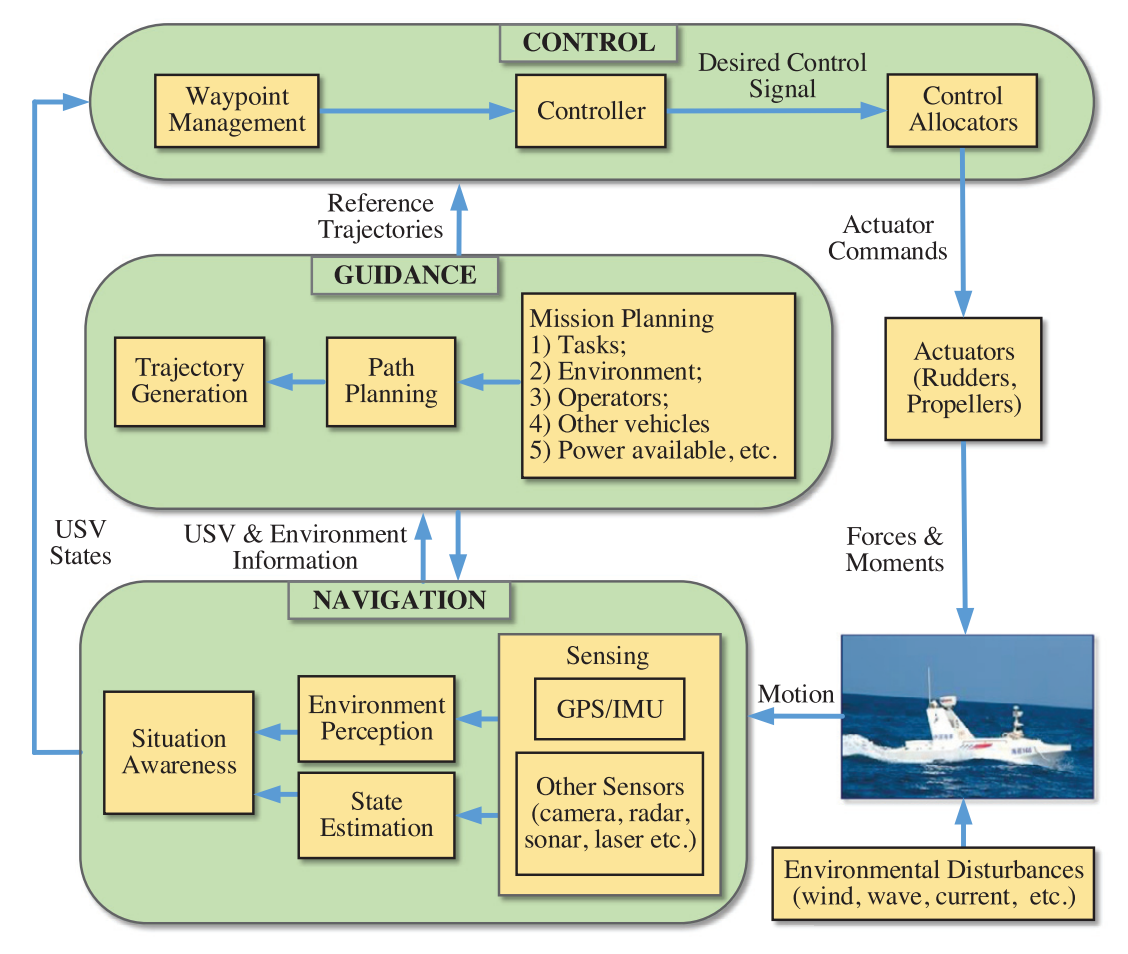
\includegraphics[scale=0.7]{figs/Liu2016Unmanned_GNCSystem.png}
        \caption{\ac{GNC} System - Components and interaction between them \cite{Liu2016Unmanned}}
        \label{fig:Liu2016Unmanned_GNCSystem}
    \end{figure}
    
    % VJ o que é importante na imagem? O que vc quer que o leitor saiba? Apontar na label e no texto. Lemre-se que vc não tem direito autoral das imagens e que isso pode virar uma dor de cabeça se o autor for chato. Sempre consulte os autores ao usar imagens de terceiros.
    
    % \subsubsection{Behavior-based systems}
        
        %% Benjamin2004COLREGS
        % The origin of behavior-based systems is commonly attributed to Brooks' "subsumption architecture" in [R. Brooks, “A Robust Layered Control System for a Mobile Robot”, IEEE Journal of Robofics and Automation, RA-2(1):14-23, April 1986]. Since then, it has been used in a large variety of applications including: indoor robots, e.g., [l, 2, 7, 9, 13, 14, 17, 19, 201, land vehicles, e.g., [16], planetary rovers, e.g., [12, 181, and marine vehicles, e.g., [3,4,6,8, 15] 
        
        %% Benjamin2004COLREGS
        % Action selection, as indicated in Fig. 1, is the process of choosing a single action for execution, given the outputs of the behaviors. The "action space" is the set of all possible distinct actions, e.g., all speed, heading and depth combinations for a marine vehicle.
        
        %% Benjamin2004COLREGS
        % Its influence depends on whether the rule associated with the behavior applies to the current situation. The output of each behavior is an objective function that rates all possible actions with respect to the corresponding COLREGS rule. The detaiIs of solving multi-objective optimization problems in the interval programming model can be found in [3]
        
    % \subsubsection{Genetic Programming}
    % Genetic Programming is an automated programming technique, based on the automated composition of 
    % a set of functional programming blocks into an increasing amount of modules for 
    % generation of a structured solution with the desired functionality. 
    % Genetic Programming explore a random combination of functional blocks through the generation of expressions 
    % tree where each node is represents a functional block. Solutions are generated by combination, mutation and
    % crossover between subtrees.
    
    % \subsubsection{A*}
    
    % The A* algorithm is a classical grid-based methodology which has been widely applied in different shapes and forms. It uses s heuristic method to focus the search towards the goal position. Using an edge cost and a heuristic based on the Euclidean distance, the A* algorithm can find the shortest paths \cite{Hart1972Formal}. For the classical A* algorithm, its scalability is limited by its memory requirements. It stores all explored nodes of a search graph in the memory, using an Open List to store nodes on the search frontier and a Closed List to store already-expanded nodes.
    
    % Depending on the size of the grid map, a large number of nodes may have to be searched at any given time. Thus, repeatedly searching through these lists can slow down the application significantly. Hence, it is not suitable for real-time engineering applications requiring on-the-fly computations.
    
    % Search space
    
    % \subsubsection{Occupancy Grid}
    % \subsubsection{Velocity Obstacle} \unsure[inline]{maybe remove from here and explain only in the literature review}
    
    % The velocity obstacle (VO) approach has been adopted by several researchers for moving hazard avoidance. Since it was first proposed in 1998 for robot motion planning [10], several extensions to VO have been made.  VO approaches generate a cone-shaped obstacle in the velocity space (hence the name velocity obstacles) and ensure that there will be no future collisions as long as the robot’s velocity vector is outside the VO. To identify the risk of future collisions, one could predict both the pose of the moving hazard and the pose of the robot for several time steps into the future, and perform collision checks using their configurations at each time slice. This approach has the advantage that it can check collisions of vehicles following arbitrary trajectories. However, because it needs to perform collision checks at many time slices, the computational load becomes very high.

    % On the other hand, VO makes a first-order (i.e., linear) prediction, and the collision check is done in the velocity space. Since a single collision check accounts for collision checks at all future times (due to the linear velocity assumption), VO is very fast to compute and extends well to high-speed operations with short reaction time. Furthermore, its simplicity is suited for our behavior-based control architecture.
    
    % \subsubsection{Line of Sight}
    % \subsubsection{Direction Priority Sequential Selection} \unsure[inline]{maybe remove from here and explain only in the literature review}
    % \subsubsection{Rule-Rapairing A*} \unsure[inline]{maybe remove from here and explain only in the literature review}
    % \subsubsection{Virtual Force Field}
    % \subsubsection{Fuzzy Logic}
    % \subsubsection{Interval Programming}
    % \subsubsection{Closest Point of Approach}
        % One is using various indicators to measure a collision risk and find associated evasive actions that keep the risk at an acceptable level. Two widely used indicators, Distance to CPA (DCPA) and Time to CPA (TCPA), are based on the concept of closest point of approach (CPA) (Kearon, 1979).
    % \subsubsection{Occupancy Grid}

\section{COLREGS}
\label{sec:colregs}

    %Campbell2012Rule
    % Human error, both active and latent, are said to cause marine collisions in an estimated 89-96\% of cases (Roth-blum (2000)), for instance the catastrophic MVDo˜na Paz ferry collision with the MTVector. An intelligent Obstacle Detection and Avoidance (ODA) system can potentially eliminate the issues caused by poor judgement or failure to react promptly.

    \ac{COLREGS}\cite{COLREGS} stands for “International Regulation for Preventing Collisions at Sea, 1972”, sometimes cited as "COLlision REGulations at Sea" or "Convention on the International Regulations for Preventing Collisions at Sea" -- in this work we adopted the latter. The definitions declared on the \ac{COLREGS} are controlled, updated and of responsibility of the \ac{IMO}. Briefly, the \ac{COLREGS} defines the rules that must be followed by vessels upon waters to avoid collision. 
    The \ac{COLREGS} are adopted by the United Nations as a global convention and must be respected by every country.
    
    The \ac{COLREGS} include 41 rules divided into five sections: General document appliance, Steering \& Sailing, Lights \& Shapes, Sound and Light Signals, and Exceptions. Relevant rules in the context of the present work are listed below. For purpose of discussion we underline subjective or ambiguous terms:
    % VJ: Em português criamos frases gigantes, em Inglês, evite isso e quebre frases que vão ficar muito grandes sempre que possível. O termo no-objective acho que se escreve sem hífen e significa: emotional; based on inner experience rather than fact. Subjective. Vc não deve usar plural ali. 
    % DJ: "Non-objective" removed.
    % Paragraph reduced.
    
    \begin{itemize}
    % VJ: penso eu que seja visto como plágio um número tão elevado de frases citadas exatamente como são. Talvez fosse melhor explicar com suas palavras.
    
    %AMA 31/1 nesse caso ae acho apropriado pois um dos objetivos de parafrasear aqui eh deixar claro alguns pontos de ambiguidade da regras. Se ele reescrevesse do jeito dele, o leitor poderia pensar q a ambiguidade eh culpa do Darlan e nao da norma. 

        \item Rule 5 - Proper "look-out" (PARAPHRASED):
        
        \begin{itemize}
            \item "Every vessel shall at all times maintain a \underline{proper look-out} by sight and hearing as well as by all available means appropriate in the prevailing circumstances and conditions so as to make a full appraisal of the situation and of the risk of collision."
        \end{itemize}
        
        This is the first rule that we detect subjectivity. The rule talks about a "proper look-out", an expression that can have a common sense between experienced sailors but it is a hard mission for system designers to address this requirement.
        
        \item Rule 6 - Safe speed (PARAPHRASED):
        
        \begin{itemize}
            \item "Every vessel shall at all times proceed at a \underline{safe speed} so that she can take proper and effective action to avoid collision and be stopped within a \underline{distance appropriate} to the prevailing circumstances and conditions."
        \end{itemize}
        
        \item Rule 7 - Risk of collision (PARAPHRASED):
        
        \begin{itemize}
            \item "Every vessel shall use \underline{all available means} appropriate to the prevailing circumstances and conditions to determine if a risk of collision exists. If there is any doubt, such risk shall be deemed to exist."
        \end{itemize}
        
        \item Rule 8 - Action to avoid collision (PARAPHRASED):
        
            \begin{itemize}
                \item "Any action to avoid collision shall be taken in accordance with the Rules of this Part and shall, if the circumstances of the case admit, be positive, made in \underline{ample time} and with due regard to the observance of \underline{good seamanship}."
                \item "Any alteration of course and/or speed to avoid collision shall if the circumstances of the case admit, be \underline{large enough} to be readily apparent to another vessel observing visually or by radar; a succession of small alterations of course and/or speed should be avoided."
                \item "If necessary to avoid collision or allow more time to assess the situation, a vessel shall slacken her speed or take all way off by stopping or reversing her means of propulsion."
            \end{itemize}
        
        \item Rule 9 - Narrow channels (PARAPHRASED):
        
            \begin{itemize}
                \item "A vessel proceeding along the course of a narrow channel or fairway shall keep as near to the outer limit of the channel or fairway which lies on her starboard side as is safe and practicable."
            
                \item "A vessel of less than 20 metres in length or a sailing vessel shall not impede the passage of a vessel which can safely navigate only within a narrow channel or fairway."
            \end{itemize}
            
            % VJ Possible implementation? Não entendi o que vc quer com estes parágrafos, melhor vc me explicar
            Possible implementation: The \ac{USV} must detect a narrow channel and the starboard-near coast and navigate near to this coast (without violation of other rules). If the system is on a \ac{USV} of less than 20 meters, it must be capable of detect other vessels and let they pass with priority on their own mission.
        
        \item Rule 10 - Traffic separation schemes (PARAPHRASED):
        
            \begin{itemize}
                \item A vessel using \ac{TSS} shall:
                \begin{itemize}
                    \item "Proceed in the appropriate traffic lane in the general direction of traffic flow for that lane."
                    \item "So far as practicable keep clear of a traffic separation line or separation zone."
                \end{itemize}
                
                \item "A vessel shall not use an inshore traffic zone when she can safely use the appropriate traffic lane within the adjacent traffic separation scheme. However, vessels of less than 20 metres in length, sailing vessels, and vessels engaged in fishing may use the inshore traffic zone." 
        
                \item "A vessel other than a crossing vessel or a vessel joining or leaving a lane shall not normally enter a separation zone or cross a separation line except:" 
                \begin{itemize}
                    \item "A vessel of less than 20 metres in length or a sailing vessel shall not impede the safe passage of a power-driven vessel following a traffic lane."          
                \end{itemize}
            \end{itemize}
            
            \ac{TSS} are defined routes, such as ground traffic lanes, with required orientation and direction. An example is presented in Figure \ref{fig:COLREGS_10_TSS_1}.
            \begin{figure}[H]
                \centering
                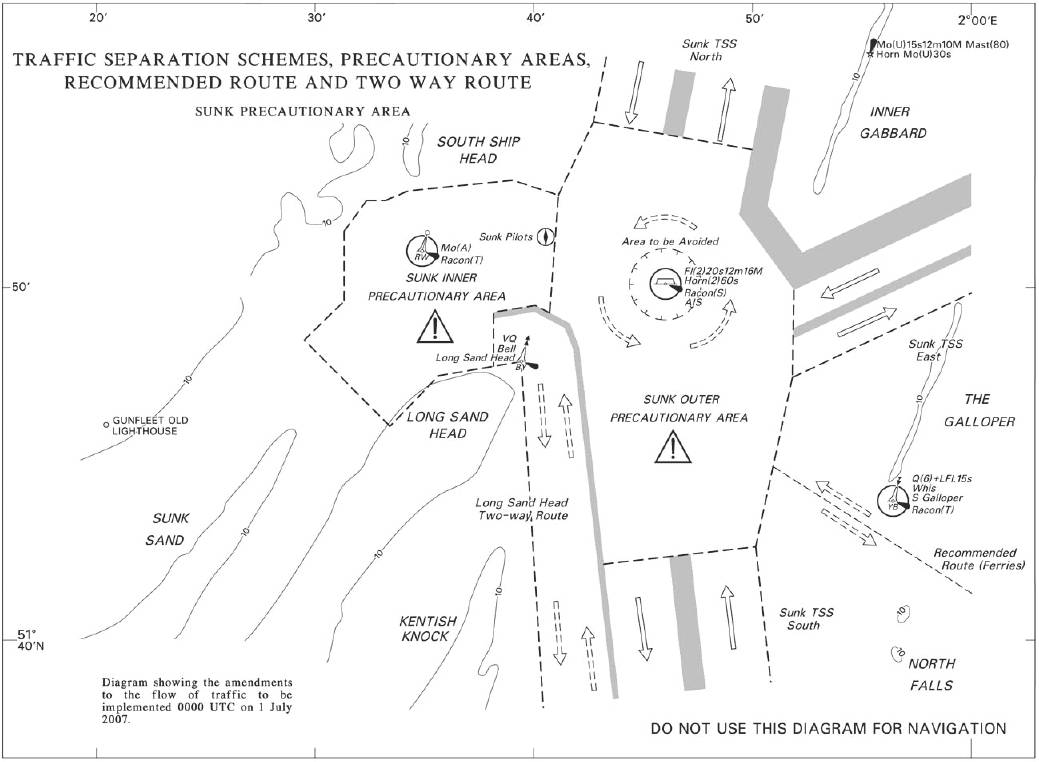
\includegraphics[scale=0.3]{figs/COLREGS_10_TSS_1.png}
                \caption{Traffic Separation Scheme Example \cite{yachtcluTSS}}
                \label{fig:COLREGS_10_TSS_1}
            \end{figure}
            
            Possible implementation: Change guidance according to \acp{TSS}.
            
        \item Rule 11 - Rules 11-18 must be followed when vessels encounters happen.
        \item Rule 13 - Overtaking (PARAPHRASED):
        
            \begin{itemize}
                \item "Any vessel overtaking any other shall \underline{keep out of the way} of the vessel being overtaken."
                \item "A vessel shall be deemed to be overtaking when coming up with another vessel from a direction more than 22.5 degrees abaft her beam, that is, in such a position with reference to the vessel she is overtaking, that at night she would be able to see only the sternlight of that vessel but neither of her sidelights."(c).
                \item "When a vessel is in any doubt as to whether she is overtaking another, she shall assume that this is the case and act accordingly."
                \item "Any subsequent alteration of the bearing between the two vessels shall not make the overtaking vessel a crossing vessel within the meaning of these Rules or relieve her of the duty of keeping clear of the overtaken vessel until she is finally past and clear."
            \end{itemize}
            
            Possible implementation: Overtaking action with degrees constraint. Detect if the \ac{USV} is being overtaken and then apply constraints to the guidance system to avoid actions that can generate dangerous situations.
            
            An example of this scenario is presented in Figure \ref{fig:COLREGS_Rule13}:
            \begin{figure}[H]
                \centering
                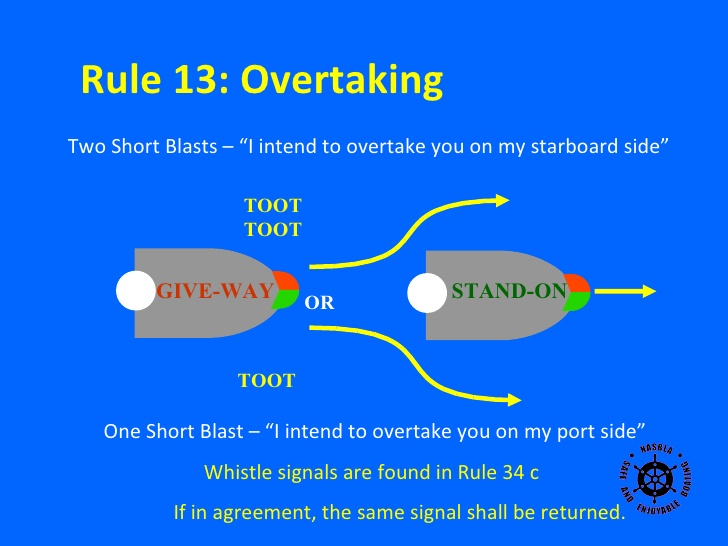
\includegraphics[scale=0.45]{figs/COLREGS_Rule13.jpg}
                \caption{Overtaking Situation \cite{nasbla2009}}
                \label{fig:COLREGS_Rule13}
            \end{figure}
            
        \item Rule 14 - Head-On (PARAPHRASED):
        
            \begin{itemize}
                \item "When two power-driven vessels are meeting on \underline{reciprocal or nearly reciprocal} courses so as to involve risk of collision each shall alter her course to starboard so that each shall pass on the port side of the other."
            \end{itemize}
            
            Possible implementation: Head-on collision avoidance action.
            
            An example of this scenario is presented in Figure \ref{fig:COLREGS_Rule14}:
            \begin{figure}[H]
                \centering
                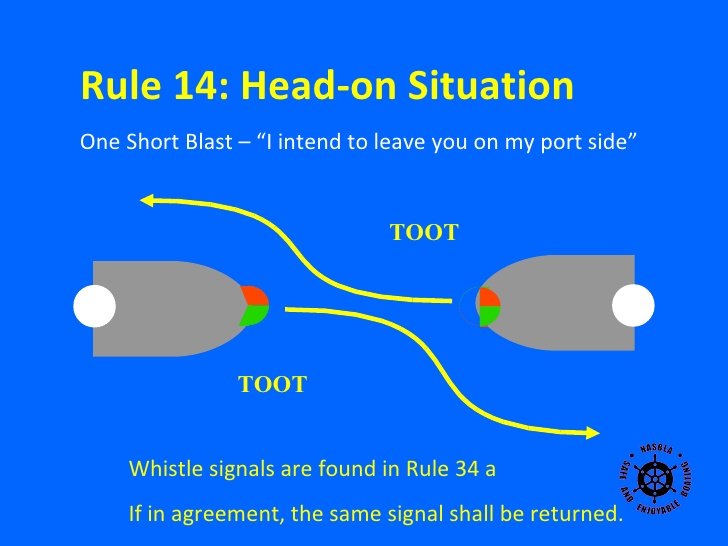
\includegraphics[scale=0.45]{figs/COLREGS_Rule14.jpg}
                \caption{Head-on Situation \cite{nasbla2009}}
                \label{fig:COLREGS_Rule14}
            \end{figure}
            
       \item Rule 15 - Crossing (PARAPHRASED):
        
            \begin{itemize}
                \item "When two power-driven vessels are crossing \underline{so as to involve risk of collision}, the vessel which has the other on her own starboard side shall keep out of the way and shall, if the circumstances of the case admit, avoid crossing ahead of the other vessel."
            \end{itemize}
            
            Possible implementation: Crossing collision avoidance action.
            
            An example of this scenario is presented in Figure \ref{fig:COLREGS_Rule15}\cite{nasbla2009}:
            \begin{figure}[H]
                \centering
                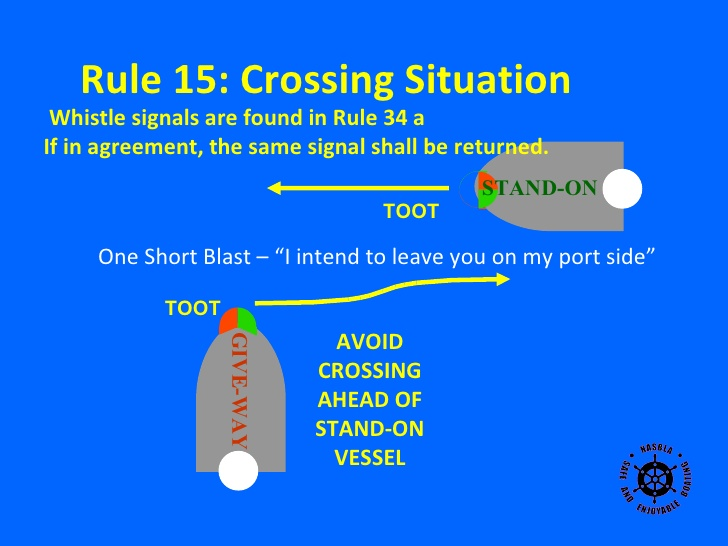
\includegraphics[scale=0.45]{figs/COLREGS_Rule15.jpg}
                \caption{Crossing Situation \cite{nasbla2009}}
                \label{fig:COLREGS_Rule15}
            \end{figure}
            
        \item Rule 16 - Action by give-way vessel (PARAPHRASED):
        
            \begin{itemize}
                \item "Every vessel which is directed to keep out of the way of another vessel shall, so far as possible, take \underline{early and substantial} action to keep \underline{well clear}."
            \end{itemize}
        
        \item Rule 17 - Action by stand-on vessel (PARAPHRASED):
        
            \begin{itemize}
                \item "Where one of two vessels is to keep out of the way the other shall keep her course and speed"
                \item "The latter vessel may however take action to avoid collision by her manoeuvre alone, as soon as it \underline{becomes apparent to her} that the vessel required to keep out of the way is not taking appropriate action in compliance with these Rules."
                \item "When, from any cause, the vessel required to keep her course and speed finds herself so close that collision cannot be avoided by the action of the give-way vessel alone, she shall take such action as will best aid to avoid collision."
            \end{itemize}
            
        \item Rule 18 - Responsibilities between vessels:
        
            There is a hierarchy of responsibilities. More powerful and robust vessels are more responsible by maneuver than less powerful or less robust. Power-driven vessel underway shall keep out of the way of a vessel not under command, a vessel restricted in its ability to maneuver, a vessel engaged in fishing, and a sailing vessel. Sailing vessel underway shall keep out of the way of a vessel not under command, a vessel restricted in its ability to maneuver, and a vessel engaged in fishing. A vessel engaged in fishing underway shall keep out of the way of a vessel not under command, and a vessel restricted in its ability to maneuver.
            
            Possible implementation: The \ac{USV} system could be capable of detecting and identify other types of vessel, this could lead to a change of action.
            
        \item Rule 23 - Power-driven vessels underway (PARAPHRASED):
        
            \begin{itemize}
                \item "A power-driven vessel underway shall exhibit:"
                \begin{itemize}
                    \item "a masthead light forward;"
                    \item "sidelights;"
                    \item "a sternlight."
                \end{itemize}   
                \item "A power-driven vessel of less than 12 metres in length may in lieu of the lights prescribed in paragraph (a) of this Rule exhibit an all-round white light and sidelights;"
                \item "A power-driven vessel of less than 7 metres in length whose maximum speed does not exceed 7 knots may exhibit an all-round white light and shall, if practicable, also exhibit sidelights;"
            \end{itemize}
            
            Possible implementation: real boat requirements for tests.
            
        \item Rule 27 - Vessels not under command or restricted in their ability to maneuver (PARAPHRASED):
        
        \begin{itemize}

            \item "A vessel not under command shall exhibit:" 
                \begin{itemize}
            
                    \item "two all-round red lights in a vertical line where they can best be seen;" 
                    \item "two balls or similar shapes in a vertical line where they can best be seen;"
                    \item "when making way through the water, in addition to the lights prescribed in this paragraph, sidelights and a sternlight."
            
                \end{itemize}
            \item "A vessel restricted in her ability to manoeuvre, except a vessel engaged in mine clearance operations, shall exhibit:"
                \begin{itemize}
        
                \item "three all-round lights in a vertical line where they can best be seen. The highest and lowest of these lights shall be red and the middle light shall be white;"
                \item "three shapes in a vertical line where they can best be seen. The highest and lowest of these shapes shall be balls and the middle one a diamond;"
        
            \end{itemize}
        \end{itemize}
        
        \item Rule 33 - Equipment for sound signals: A vessel of less than 12 meters in length shall be provided with some means of making an efficient sound signal.

    \end{itemize}
    
    The highlighted rules above will be used in the research proposal of this document. 
    From them we can have a glance of the non-objectiveness or ambiguity of some terms used for rules definition such as proper look-out", "safe speed", "ample time", "large enough", and others. Some rules are related to possible or mandatory features required for a \ac{USV} system, such as 9, 10, 13, 14, 15, 16, 17, and 18. Also, other rules are related to structural requirements for \ac{USV}s in real-world trials, such as 23, and 33.
    
    \ac{COLREGS} rules were not defined considering autonomous systems such as \ac{USV}s. They were written to be interpreted by well-experienced sailors and imply usage of their experience and common sense. There are gaps to be filled and subjective or ambiguous definitions to be addressed, making the development of a \ac{COLREGS}-compliant \ac{USV} guidance system challenging.
    % VJ: reorganizar

    \subsection{Surface Vehicle Modeling}
    \subsection{Configuration Space}
    \subsection{Planning Algorithms}